\documentclass[a4paper,11pt,oneside]{book}

% packages 
\usepackage{arsclassica}    % fancy layout
\usepackage[english]{babel}\addto{\captionsenglish}{\renewcommand{\bibname}{References}}
\usepackage{caption}         % figure captions
\usepackage[square,numbers,super,sort&compress]{natbib}  % bibliography style
\usepackage[cc]{titlepic}    % enable logo on title page
\usepackage{graphicx}       % logo related
\usepackage{multirow}

\usepackage{standalone}
\standalonetrue

% Margins for pretty version ::
%\usepackage[pass]{geometry}
% Margins for university regulations ::
\usepackage[top=2cm, bottom=4cm, left=4cm, right=2.5cm]{geometry}
\usepackage{setspace}
\onehalfspacing

% don't hang captions
\captionsetup{format=plain}

% bibliography
\bibliographystyle{../thesis}

% title setup
\title{ \vspace{3in} Unravelling higher order genome organisation {\small [working
    title]} \\ \vspace{2em} {\large {\bf Results 5: Collaborations}} }
\author{Benjamin L. Moore}
\titlepic{\vspace{2.2in} 
\includegraphics[width=\textwidth]{/Users/benmoore/hvl/1yrReport/figs/igmm.png}}

\begin{document}

%\maketitle

\chapter{Local chromatin conformation}\label{chap:shh}

\section{Introduction}

The Hi-C assay provides a genome-wide overview of chromatin conformation, however this broad scope imposes resolution limits inherent to an all-vs-all assay. For a closer look at chromatin conformation within a region of interest, alternative C-based assays such as 3C, 4C and 5C can be employed alongside classical microscopy techniques like FISH.

Here I discuss two collaborative projects involving the use of 4C and 5C data to "zoom in" on two well-studied regions related to limb development: the ZRS enhancer and HoxD gene cluster.

\section{4C at the SHH locus}\label{sec:4cshh}

\begin{figure}
\begin{center} 
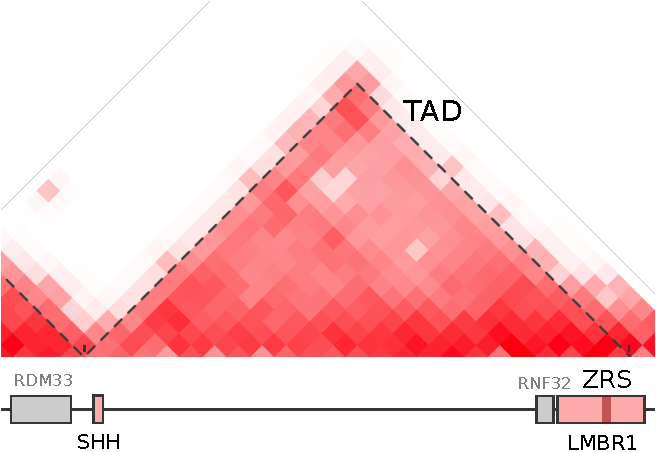
\includegraphics[width=3.5in]{figs/shhtad.pdf}
\captionsetup{width=\textwidth} 
\caption[SHH--ZRS contacts occur within a stable TAD.]{ {\bf SHH--ZRS contacts occur within a stable TAD. }
An approximately 1 Mb region of the mouse genome is shown below a Hi-C contact map (derived from previously published data\cite{Dixon2012}). A clear TAD can be identified spanning from SHH to ZRS, dashed lines show TAD boundaries called by \citet{Dixon2012}. This figure was generated for \citet{Anderson2014a}.
}\label{fig:shhtad}
\end{center} 
\end{figure} 

% , and is conserved across mammals and fish

Anterior-posterior patterning in the developing limb is regulated in mammals by \emph{Sonic hedgehog} (SHH).\cite{Anderson2012} Specifically, the SHH gene is expressed within a confined region named the "zone of polarising activity". Its expression within this region is known to be regulated by a well-studied enhancer, the "zone of polarising activity regulatory sequence" or ZRS.\cite{Hill2013a} ZRS is located almost 1 Mb downstream of its target SHH promoter in humans, and is located in intronic regions of another gene, LMBR1 (Fig. \ref{fig:shhtad}).\cite{Hill2013a, Laurell2012} Single point mutations and short insertions within this enhancer have been linked to various limb deformities, including pre- and post-axial polydactyly.\cite{Anderson2012, Lettice2008, Laurell2012} For example, a heritable point mutation in the ZRS enhancer is the cause of polydactyly in "Hemingway cats", a large group of domestic cats with extra toes that reside at the former home of Ernest Hemingway.\cite{Lettice2008}  

Collaborators have developed a model system which allows inducible SHH expression in a non-expressing 14fp cell line derived from the developing limb bud. Application of trichostatin A (TSA) then leads to detectable SHH expression, and increased levels of the histone activation mark H3K27ac at the ZRS (\emph{unpublished data}). However, the question remains whether this TSA treatment is fundamentally altering local chromatin structure, that is, bringing together the ZRS enhancer with its target SHH promoter, or whether ZRS and SHH are in contact in both the active and non-expressing cell lines and SHH expression is blocked through other means. Analysis of the region through FISH implies similar levels of compaction in SHH expressing and non-expressing cells (\emph{data not shown}), suggesting the latter explanation. Additionally, studies have previously reported the SHH--ZRS interaction is an example of a "pre-formed loop", and as such is maintained regardless of transcriptional activity.\cite{Bouwman2015a}

My part in this collaboration was to analyse 3C-seq (also known as 4C) data generated by our collaborators for the SHH--ZRS region in mouse. Additionally, the 4C procedure\cite{Stadhouders2013} was adapted for specific in-house sequencing instruments (an Ion Torrent Ion Proton\textsuperscript{TM} sequencer as opposed to Illumina\textsuperscript{TM} technology) and as such required diagnostics to confirm the experimental data was accurate. 

\subsection{4C pipeline}

The 4C analysis pipeline, starting from de-multiplexed \texttt{fastq} files as produced by our in-house sequencing facilities, can be summarised as:

\begin{enumerate}
\item Trim known bait sequence using \texttt{cutadapt},\cite{cutadapt} select only those reads where known sequence was present
\item Map reads to reference genome \texttt{mm9} using \texttt{bowtie2}\cite{Langmead2012} with the \texttt{very-sensitive} flag
\item Filter alignments with a MAPQ score $<30$ to select for high-confidence alignments using \texttt{samtools}\cite{Li2009}
\item Normalise and analyse contacts using the \texttt{r3cseq} R package (Methods \ref{methods:4c})
\end{enumerate}

% Adam sent a powerpoint he gave for section meeting, see also Prof Hill's publications

\subsection{Analysis of ZRS interactions}

\begin{figure}
\begin{center} 
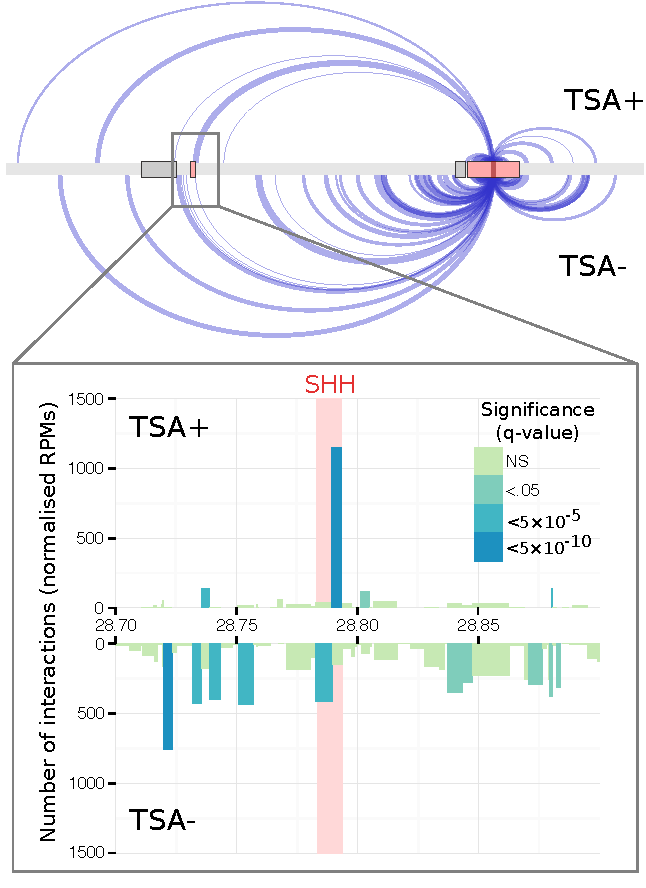
\includegraphics[width=5in]{figs/shharc_full.pdf}
\captionsetup{width=\textwidth} 
\caption[TSA treatment induces a strong ZRS--SHH interaction. ]{ {\bf TSA treatment induces a strong ZRS--SHH interaction. }
4C interactions are shown as edges from source node (ZRS enhancer bait fragment) to targets along an approximately 2 Mb region of chromosome 5. Edge width is proportional to the number of interactions, only highly significant interactions are shown (FDR $q$-value $<5 \times 10 ^{-5}$). Zoomed region shows the number of interactions of the bait region with SHH in both untreated and TSA treated (after 18h) samples. Each rectangle is a restriction fragment, coloured by FDR $q$-value indicating the significance of the interaction above expected levels.
}\label{fig:ssharc}
\end{center} 
\end{figure} 

4C experiments were performed by collaborators using the ZRS region as a bait sequence, or "viewpoint", such that it contacts were measured with all other HindIII restriction fragments genome-wide. 4C was performed in both untreated and non-SHH expressing cells (\emph{TSA--}) and in cells treated with TSA, thereby causing SHH expression (\emph{TSA+}). 

The first stage in analysing these contacts is to convert observed raw sequencing reads to normalised frequencies (Methods \ref{methods:4cnorm}), these normalised values are then assigned significance scores in the form of $q$-values, with the aim of finding those significantly over-represented relative to expectation (Methods \ref{methods:4csignif}).

The results of a comparison between TSA treated and untreated samples is shown in Figure \ref{fig:ssharc}. In it we see a striking and highly significant ZRS--SHH contact in the treated sample ($q$-value $ < 5 \times 10^{-10}$), with a weaker but still significant contact in the adjacent restriction fragment in the untreated sample ($q$-value $ < 5 \times 10^{-5}$). 

We also see more broadly a much higher total number of significant contacts in the untreated sample around the viewpoint (Fig. \ref{fig:4carcs}). In the treated samples, only a few contacts cross the stringent $q$-value threshold, with the SHH--ZRS contact among the most significant in terms of both $q$-value and supporting number of reads (indicated by the thickness of the arc, Figs. \ref{fig:ssharc}, \ref{fig:4carcs}).

Existing multi-probe FISH data produced by our collaborators shows approximately equal levels of compaction in this region in both TSA treated and untreated cells (\emph{data not shown}). This information in combination with the 4C results reported here (Fig. \ref{fig:ssharc}) support a hypothesis that while both samples are held together in a TAD (Fig. \ref{fig:shhtad}) --- unavoidably inducing many contacts --- it is only in the treated sample where a highly-specific ZRS--SHH contact occurs and potentially is then bring about expression of the \emph{SHH} gene.

% Conclusions: appears ZRS contacts become more targetted in TSA+ cells, before more diffuse. 
% Maybe in contact all the time (supported by FISH data) but not engaging in specific contacts when non-expressing.

\begin{figure}
\begin{center} 
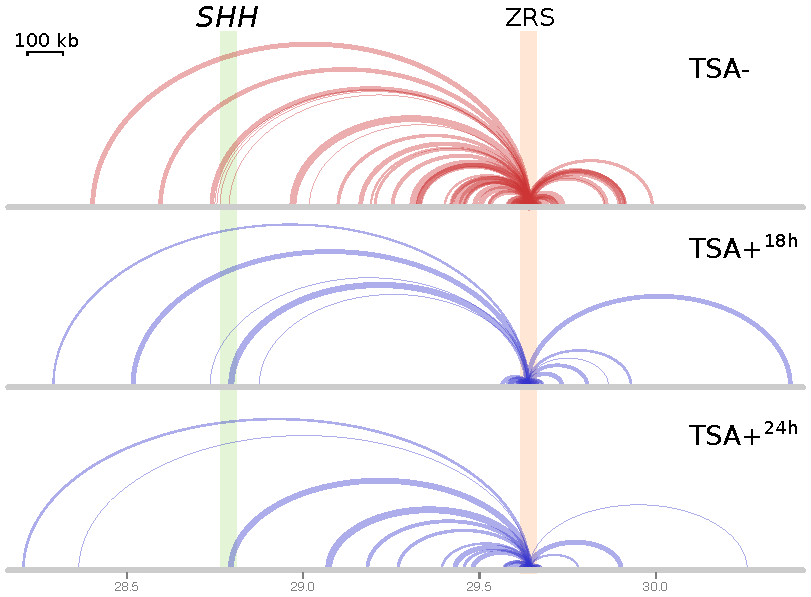
\includegraphics[width=5in]{figs/4c_arcs.pdf}
\captionsetup{width=\textwidth} 
\caption[ A stable ZRS--SHH interaction is coupled with reduced extraneous contacts. ]{ {\bf A stable ZRS--SHH interaction is coupled with reduced extraneous contacts. }
Arc plots are shown for an untreated, non-expressing 14fp cell population (\emph{untreated}) and following TSA treatment after 18 and 24 hours. Arcs link highly significant interactions ($q$-value $< 5 \times 10^{-5}$) and arc widths are proportional to the normalised number of reads recorded for the interaction (Methods \ref{methods:4c}).
}\label{fig:4carcs}
\end{center} 
\end{figure} 

%\subsection{4C / Hi-C comparison}
%
%Hi-C data in mouse cells has been previously published,\cite{Dixon2012} so can be compared with this novel 4C data to give broader contextual information about chromatin conformation in the region under study.

\subsection{Assay diagnostics}

The 4C protocol used by our collaborators in this work was that of \citet{Stadhouders2013}. In it, the authors advise some statistical tests to ensure the quality of the experiment results. Among these were:\cite{Stadhouders2013}

\begin{enumerate}
\item Sequencing reads should be found to have high duplication rates of $95\%$ or greater.
\item $50\%$ or more of all reads should map to the chromosome on which the bait region is located.
\end{enumerate}

% duplication: treated 02 : 71.2 % (reads 42.2M)
%                                 04 : 84.4 % (reads 24.2M)
%                    haeiii: 74.0% (reads 10.4M)
%                    mluci: 62.8% (reads 10M)

Sequence duplication levels were measured with \texttt{FastQC}\cite{fastqc} and are shown in Table \ref{tab:4c}. We find slightly lower than expected levels of duplication, ranging from $62.8\%$ to $84.4\%$. This suggests that while the assay does appear to be working, there may be extraneous noise and non-bait interactions in the sequencing library.

\begin{table}[]
\centering
\caption[4C sequencing library statistics.]{ {\bf 4C sequencing library statistics.}
4C experiments are summarised as total number of reads in each experiment and the percentage of those reads labelled "duplicates". Note in 4C these duplicates are not artifactual and instead result from large numbers of contacts nearby to the viewpoint.
}
\label{tab:4c}
\begin{tabular}{lcccc}
                                      & \multicolumn{2}{c}{{\bf TSA-}}      & \multicolumn{2}{c}{{\bf TSA+}}   \\ \cline{2-5} 
\multicolumn{1}{l|}{}                 & MlucI & \multicolumn{1}{c|}{HaeIII} & 18h  & \multicolumn{1}{c|}{24h}  \\ \hline
\multicolumn{1}{|l|}{Reads (Million)} & 10    & \multicolumn{1}{c|}{10.4}   & 42.2 & \multicolumn{1}{c|}{24.2} \\ \cline{2-5} 
\multicolumn{1}{|l|}{Duplicated (\%)} & 62.8  & \multicolumn{1}{c|}{74.0}   & 71.2 & \multicolumn{1}{c|}{84.4} \\ \hline
\end{tabular}
\end{table}

We found the proportion of reads mapped to the fair region chromosome, chromosome 5 in this case, fell below the prescribed level of $50\%$. Looking at three experiments (two from the untreated control), we find instead that between approximately $10$--$20\%$ of all reads mapped to the bait chromosome (Fig. \ref{fig:4cchromosomes}). While this is still a clear enrichment over non-bait chromosomes, it suggests the assay results suffer from either increased \emph{trans}-contact noise or decreased \emph{cis}-contact enrichment around the bait region. 

\begin{figure}
\begin{center} 
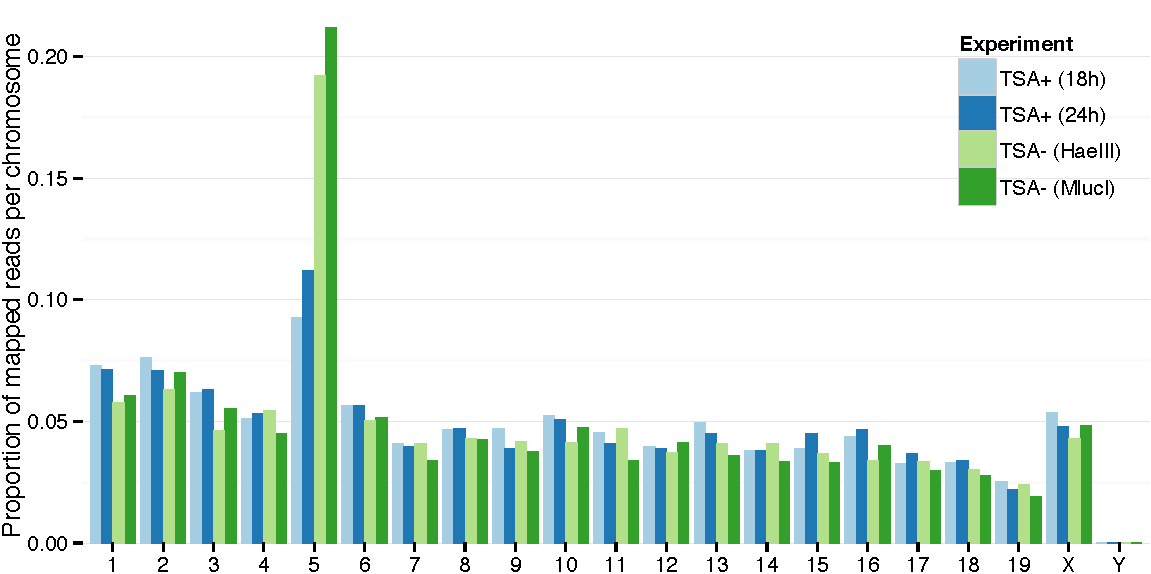
\includegraphics[width=5.4in]{figs/4c_chromosomes.pdf}
\captionsetup{width=\textwidth} 
\caption[ The bait chromosome is enriched for 4C sequencing reads. ]{ {\bf The bait chromosome is enriched for 4C sequencing reads. }
Chromosome 5 is visibly enriched for 4C reads as it  contains the ZRS bait region (or viewpoint). Untreated control samples (\emph{TSA-}) were assayed with two different secondary restriction enzymes (4-cutters HaeIII and MlucI).
}\label{fig:4cchromosomes}
\end{center} 
\end{figure} 

Lower than expected levels of both sequence duplication and bait chromosome enrichment suggest loss of signal around the bait region itself. This is the area where we'd expect both very high levels of duplication (identical restriction fragment pairings between nearby genomic locations) and a majority of all sequencing reads, driving the overall chromosome enrichment. The precise reason for the discrepancy is unclear but suggests the results may have a lower signal-to-noise ratio than has previously been achievable in 4C experiments.\cite{Stadhouders2013} Potentially the signal-to-noise ratio could be improved by utilising a double cross-linking procedure such as that used in \citet{Lin2012}

\section{3D modelling of chromatin fibre}

% intro stuff introducing 3d modelling
Chromosome conformation capture allow investigation of genome organisation, but such data are commonly analysed using one or two-dimensional representations. A growing set of algorithms looks instead to rebuild the three-dimensional polymer trajectory of a chromatin fibre, using Hi-C or 5C data as input (e.g. \citenum{Bau2011a, Hu2013a, Varoquaux2014a, Lesne2014, Trieu2014, Peng2013, Ay2014b, Caudai2015}). Intuitively, in each method the interaction frequency between two regions is idealised as inversely proportional to their physical distance (where possible and according to various other constraints). Where these methods differ is in their approaches to solving this optimisation problem. We chose the \texttt{AutoChrom3D} method\cite{Peng2013} for use in this work (described in Section \ref{sec:achrom}) as the algorithm can accept 5C input and model polymers at high resolution of 8 kb or greater.

\subsection{\texttt{AutoChrom3D} method}\label{sec:achrom}

The procedure implemented in \texttt{AutoChrom3D} can be summarised as:\cite{Peng2013}

\begin{enumerate}
\item The chromatin fibre is represented as beads-on-a-string, with $N_{beads} = \lceil\frac{L}{R}\rceil$ (where $L$ is the length of the region and $R$ the resolution)
\item A local compaction parameter is calculated using a sliding window of each 50 adjacent beads (intra-window contacts are averaged and compared to those over the whole region under study)
\item Interaction frequency between beads of a given genomic distance is modelled as a Poisson-distributed random variable and noisy or unstable contacts, considered in the context of neighbouring beads, are filtered
\item This filtered set of interaction frequencies are then normalised using the previously-calculated compaction parameter to give an $N_{beads} \times N_{beads}$ matrix of interaction strengths
\item Interaction strength is converted to spatial distance through two linear transformations based on experimental observations of nuclear occupancy and regional flexibility\cite{Kalhor2012}
\item Cartesian co-ordinates are then calculated via non-linear constrained optimisation of pairwise spatial distances using LINGO\cite{lingo}
\end{enumerate}

\subsection{Modelling the \emph{Shh} region with 5C}\label{sec:shh5c}

5C data was generated by our collaborators over the same \emph{Shh}--ZRS region as was assayed with 4C (Fig. \ref{fig:shhtad}; Section \ref{sec:4cshh}) with the aim of developing a multi-point perspective on local chromatin conformation beyond that available from 4C data.

We used this 5C experimental data in combination with a particular three-dimensional inference program  (\texttt{AutoChrom3D}\cite{Peng2013}) in an attempt to compare polymer trajectories in TSA treated and untreated 88fp mouse cells, a similar and complimentary cell line to that used in earlier 4C experiments (14fp). As a control, 5C was also performed on mandibular (MD) cells, with and without TSA treatment, which do not express \emph{Shh}. Prior to structural modelling, the \texttt{my5C} program was used to generate normalised 5C interaction frequencies.\cite{Lajoie2009a}

\begin{figure}
\begin{center} 
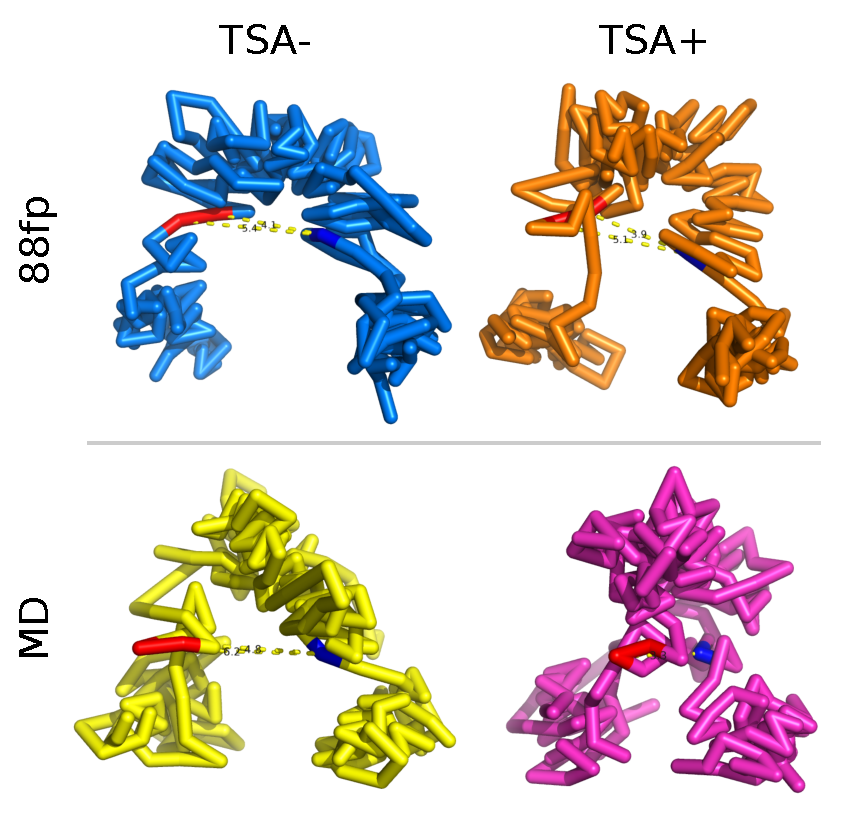
\includegraphics[width=5.45in]{figs/5c3d.pdf}
\captionsetup{width=\textwidth} 
\caption[ Inferred polymer trajectories of the ZRS--SHH region following TSA treatment in two cell lines. ]{ {\bf Inferred polymer trajectories of the ZRS--SHH region following TSA treatment in two cell lines. }
3D structures are shown for 5C experiments assaying the region around \emph{Shh} (\emph{red}) and ZRS (\emph{blue}) in an \emph{Shh}-expressing limb bud cell line (88fp) and a non-expressing mandibular cell line (MD). Labelled measurements are given in Table \ref{tab:3ddist}. Structures were predicted by \texttt{AutoChrom3D}\cite{Peng2013} using $210 \times 8$ kb beads per polymer.
}\label{fig:5c3d}
\end{center} 
\end{figure} 

We find that TSA treatment of 88fp cells does appear to slightly reduce the distance between \emph{Shh} and ZRS in inferred 3D structures (Fig. \ref{fig:5c3d}), however this difference is overshadowed---to our surprise---by that observed in the non-expressing MD cell line. This latter mandibular cell line undergoes a large structural transition which brings together the \emph{Shh} gene and the ZRS enhancer. Measurements between these elements for each structure are shown in Table \ref{tab:3ddist}.

We also report a greater overall structural shift following TSA treatment in the MD cell line, with an RMSD between the two structures of $2.377$ arbitrary units, relative to $1.701$ between TSA+ and TSA- 88fp cells. The radius of gyration, unchanged in 88fp, is also decreased in the MD cell line following TSA treatment, indicating the region becomes more compact following TSA treatment (Table \ref{tab:3ddist}).

\begin{table}[]
\centering
\caption[Measurement distances between ZRS and SHH in each inferred 3D structure.]{ {\bf Measurement distances between ZRS and SHH in each inferred 3D structure. }
Distances are given in arbitrary units. \emph{Shh} spans two beads of the polymer model, hence two distances are calculated in each case ($d_1$, $d_2$). RMSD is the minimised root mean squared deviation between the two structures and is given as a relative unitless quantity. The radius of gyration (gyradius) is also shown.
}
\label{tab:3ddist}
\begin{tabular}{ll|cc|l|cc|}
                      &    & \multicolumn{2}{c|}{{\bf Distance}} & \multirow{2}{*}{RMSD}   & \multicolumn{2}{c|}{{\bf Gyradius } ($\mu$m)}             \\
                      &    & TSA-             & TSA+             &                        & TSA-                   & TSA+                   \\ \hline
\multirow{2}{*}{88fp} & $d_1$ & 5.4              & 5.1              & \multirow{2}{*}{1.701} & \multirow{2}{*}{0.244} & \multirow{2}{*}{0.244} \\
                      & $d_2$ & 4.1              & 3.9              &                        &                        &                        \\ \hline
\multirow{2}{*}{MD}   & $d_1$ & 6.2              & 3.3              & \multirow{2}{*}{2.377} & \multirow{2}{*}{0.217} & \multirow{2}{*}{0.205} \\
                      & $d_2$ & 4.8              & 2.0              &                        &                        &                        \\ \hline
\end{tabular}
\end{table}

\subsection{Repeat simulations}

We have shown what appears to be a structural shift in the \emph{Shh}-ZRS locus per 3D modelling predictions (Section \ref{sec:shh5c}). It is of interest to assess the stability and reproducibility of these results through repeat simulations of the polymer trajectory. At this point it is unclear whether the \emph{Shh}-ZRS bound state represents a firm consensus over the cell population, or an alternative structure with similar optimisation energy to that of the more non-bound state. 

%Due to the use of cell populations we cannot resolve whether such a contact is either constitutive in a certain proportion of cells under study, or an ephemeral yet commonly-occurring interaction.

We re-ran simulations of the 3D chromatin fibre in the \emph{Shh}-ZRS region a total of five times (Fig. \ref{fig:3dreps}). In every case, the algorithm generates the known \emph{Shh}-ZRS TAD as a compacted domain bookended by the two loci under study. This sanity check ensures the results are broadly compatible with our \emph{a prior} expectation of the region's structure given the 2D heatmap representation of 5C data (Fig. \ref{fig:shhtad}).

\begin{figure}
\begin{center} 
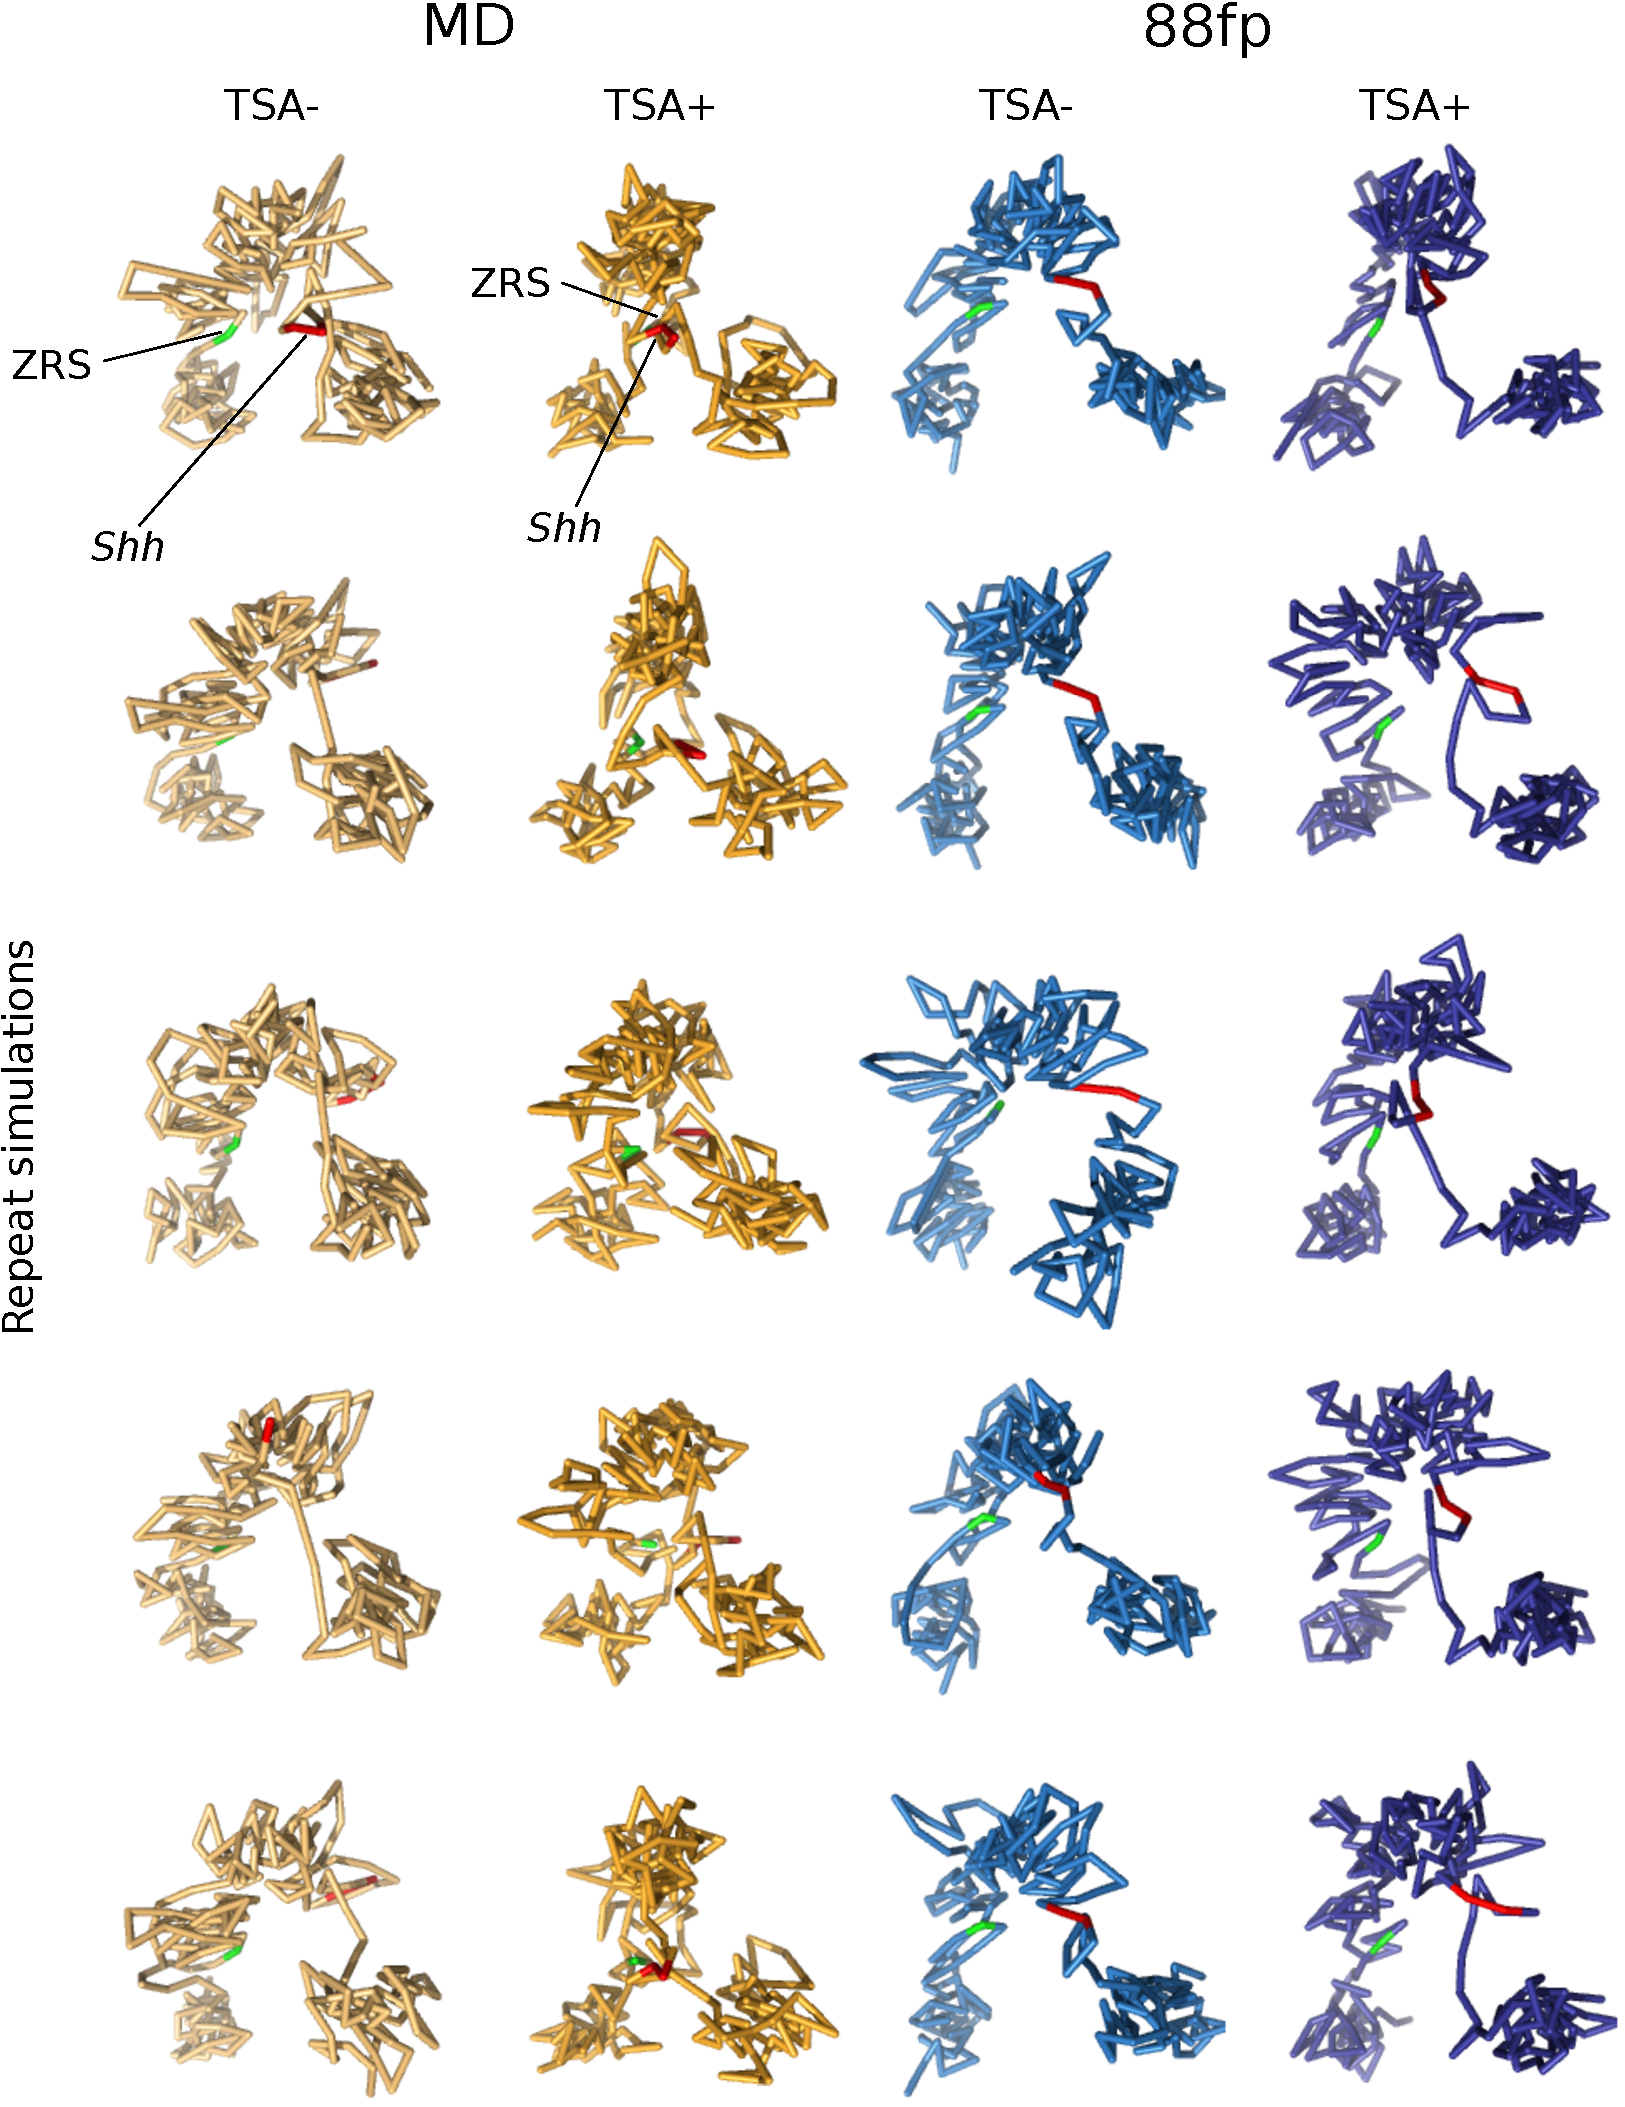
\includegraphics[width=5.45in]{figs/3dreps.pdf}
\captionsetup{width=\textwidth} 
\caption[ Repeat simulations of 3D polymer trajectories in the \emph{Shh}--ZRS region. ]{ {\bf Repeat simulations of 3D polymer trajectories in the \emph{Shh}--ZRS region. }
3D structures are shown for 5C experiments assaying the region around \emph{Shh} (\emph{red}) and ZRS (\emph{blue}) in an \emph{Shh}-expressing limb bud cell line (88fp) and a non-expressing mandibular cell line (MD). Structures were aligned as whole molecules with the uppermost replicate in each column.
}\label{fig:3dreps}
\end{center} 
\end{figure} 

\begin{figure}
\begin{center} 
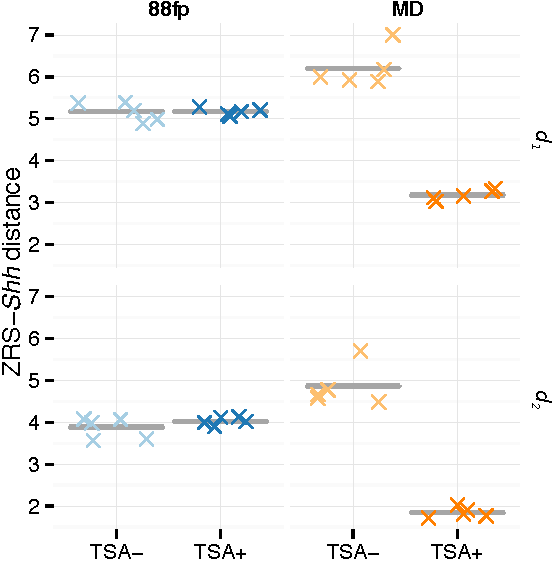
\includegraphics[width=2.75in]{figs/3d_dists.pdf}
\captionsetup{width=\textwidth} 
\caption[ \emph{Shh}--ZRS distance measurements from repeated 3D polymer simulations. ]{ {\bf \emph{Shh}--ZRS distance measurements from repeated 3D polymer simulations. }
Measurements were taken from 5 replicate 3D simulations (shown in Fig. \ref{fig:3dreps}). Distances are given in arbitrary units. \emph{Shh} spans two beads of the polymer model, hence two distances are calculated in each case ($d_1$, $d_2$).
}\label{fig:3ddist}
\end{center} 
\end{figure} 

%\section{5C in the HoxD region}
%
%HoxD is another well-studied genetic system involved in limb development and under the control of known enhancers. In this experiment, our collaborators were interested in the chromatin conformations of HoxD13 loci in both the anterior and posterior developing limb bud, particularly how and where the two differed. To this end, our collaborators performed 5C for two biological replicates in anterior and posterior limb bud cell lines, and my contribution was to call differential contacts between the two conditions.
%
%% Region gets a mention in Bickmore 2013 review 
%
%% files for this under iain on ext HD
%% relevant publications: http://dev.biologists.org/content/139/17/3157.full.pdf+html
%
%%Iain's thesis: https://www.era.lib.ed.ac.uk/handle/1842/8056
%
%\subsection{Differential contacts}
%
%% raw diff: fold change?
%
%\begin{figure}
%\begin{center} 
%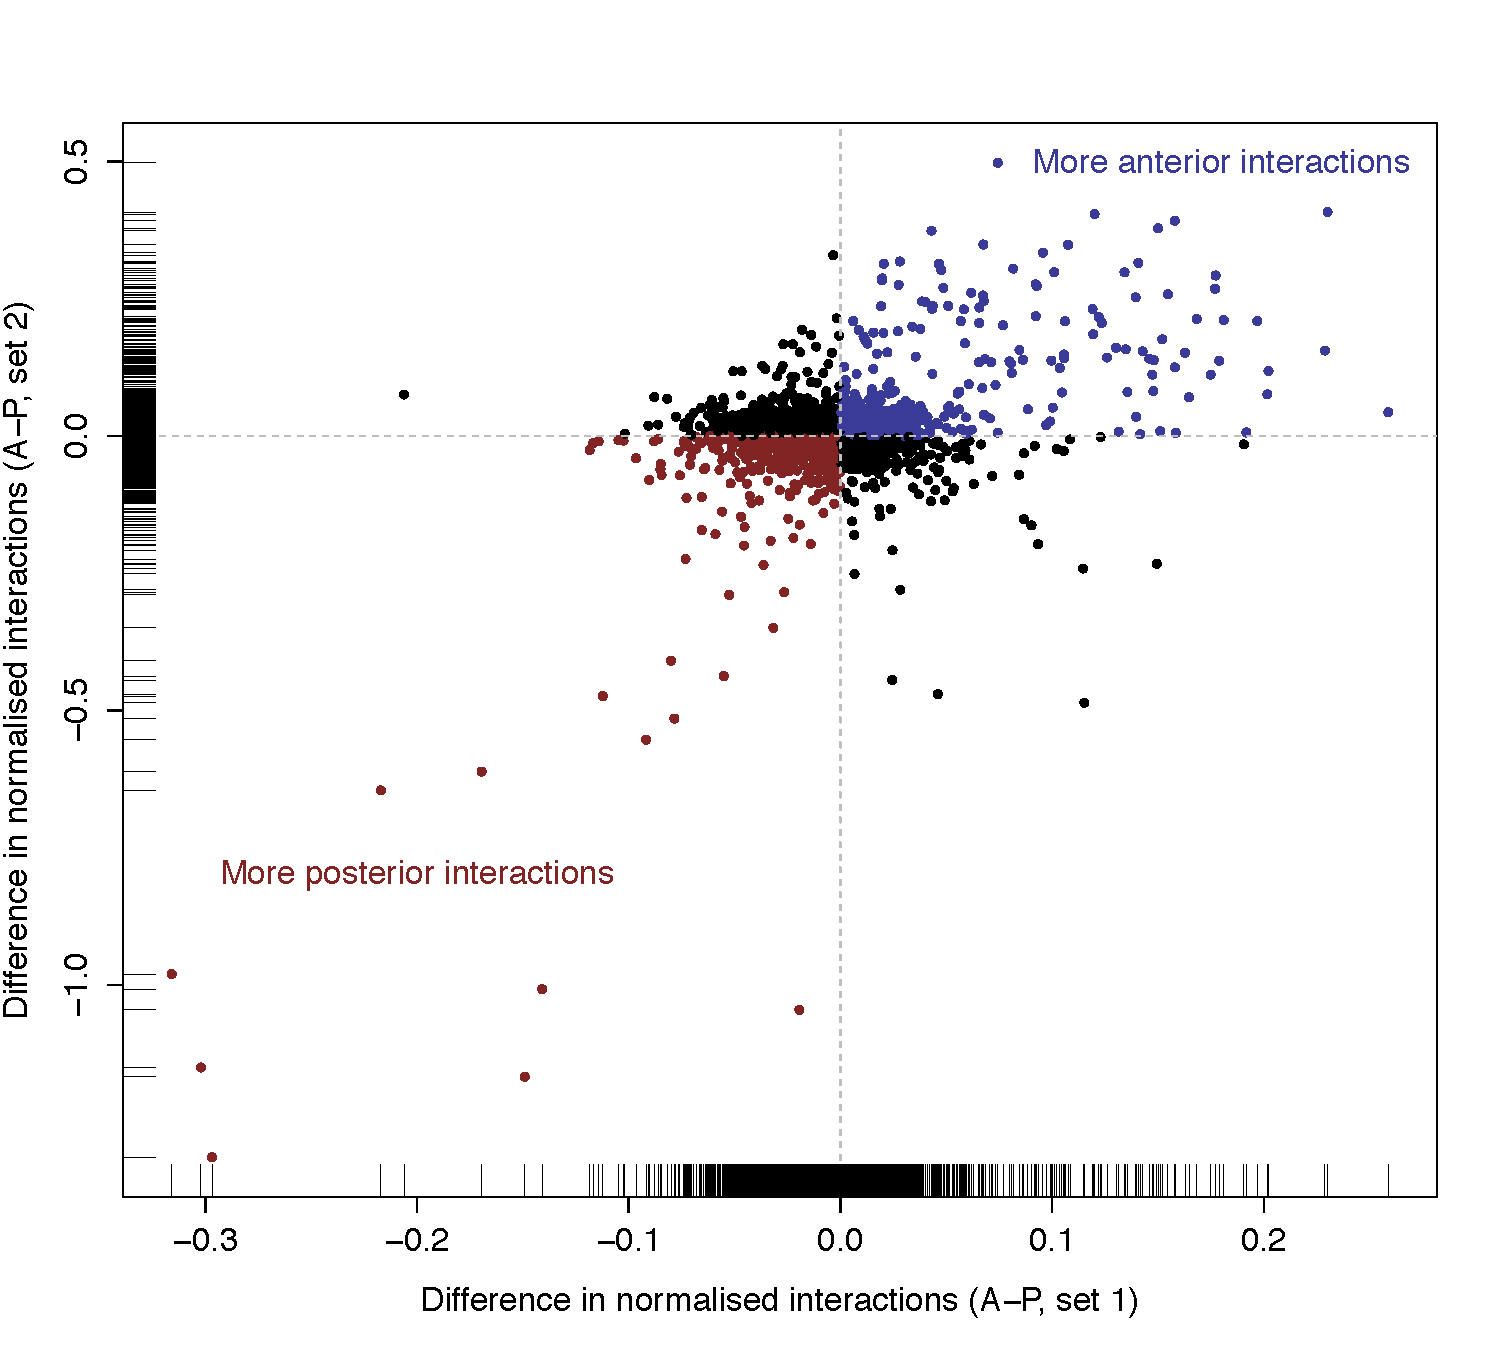
\includegraphics[width=\textwidth]{figs/5cfc.pdf}
%\captionsetup{width=\textwidth} 
%\caption[Raw differences between anterior and posterior 5C interactions.]{ {\bf Raw differences between anterior and posterior 5C interactions. }
%Placeholder
%}\label{fig:5cfc}
%\end{center} 
%\end{figure} 
%
%% statistical test of differential contacts
%
%\begin{figure}
%\begin{center} 
%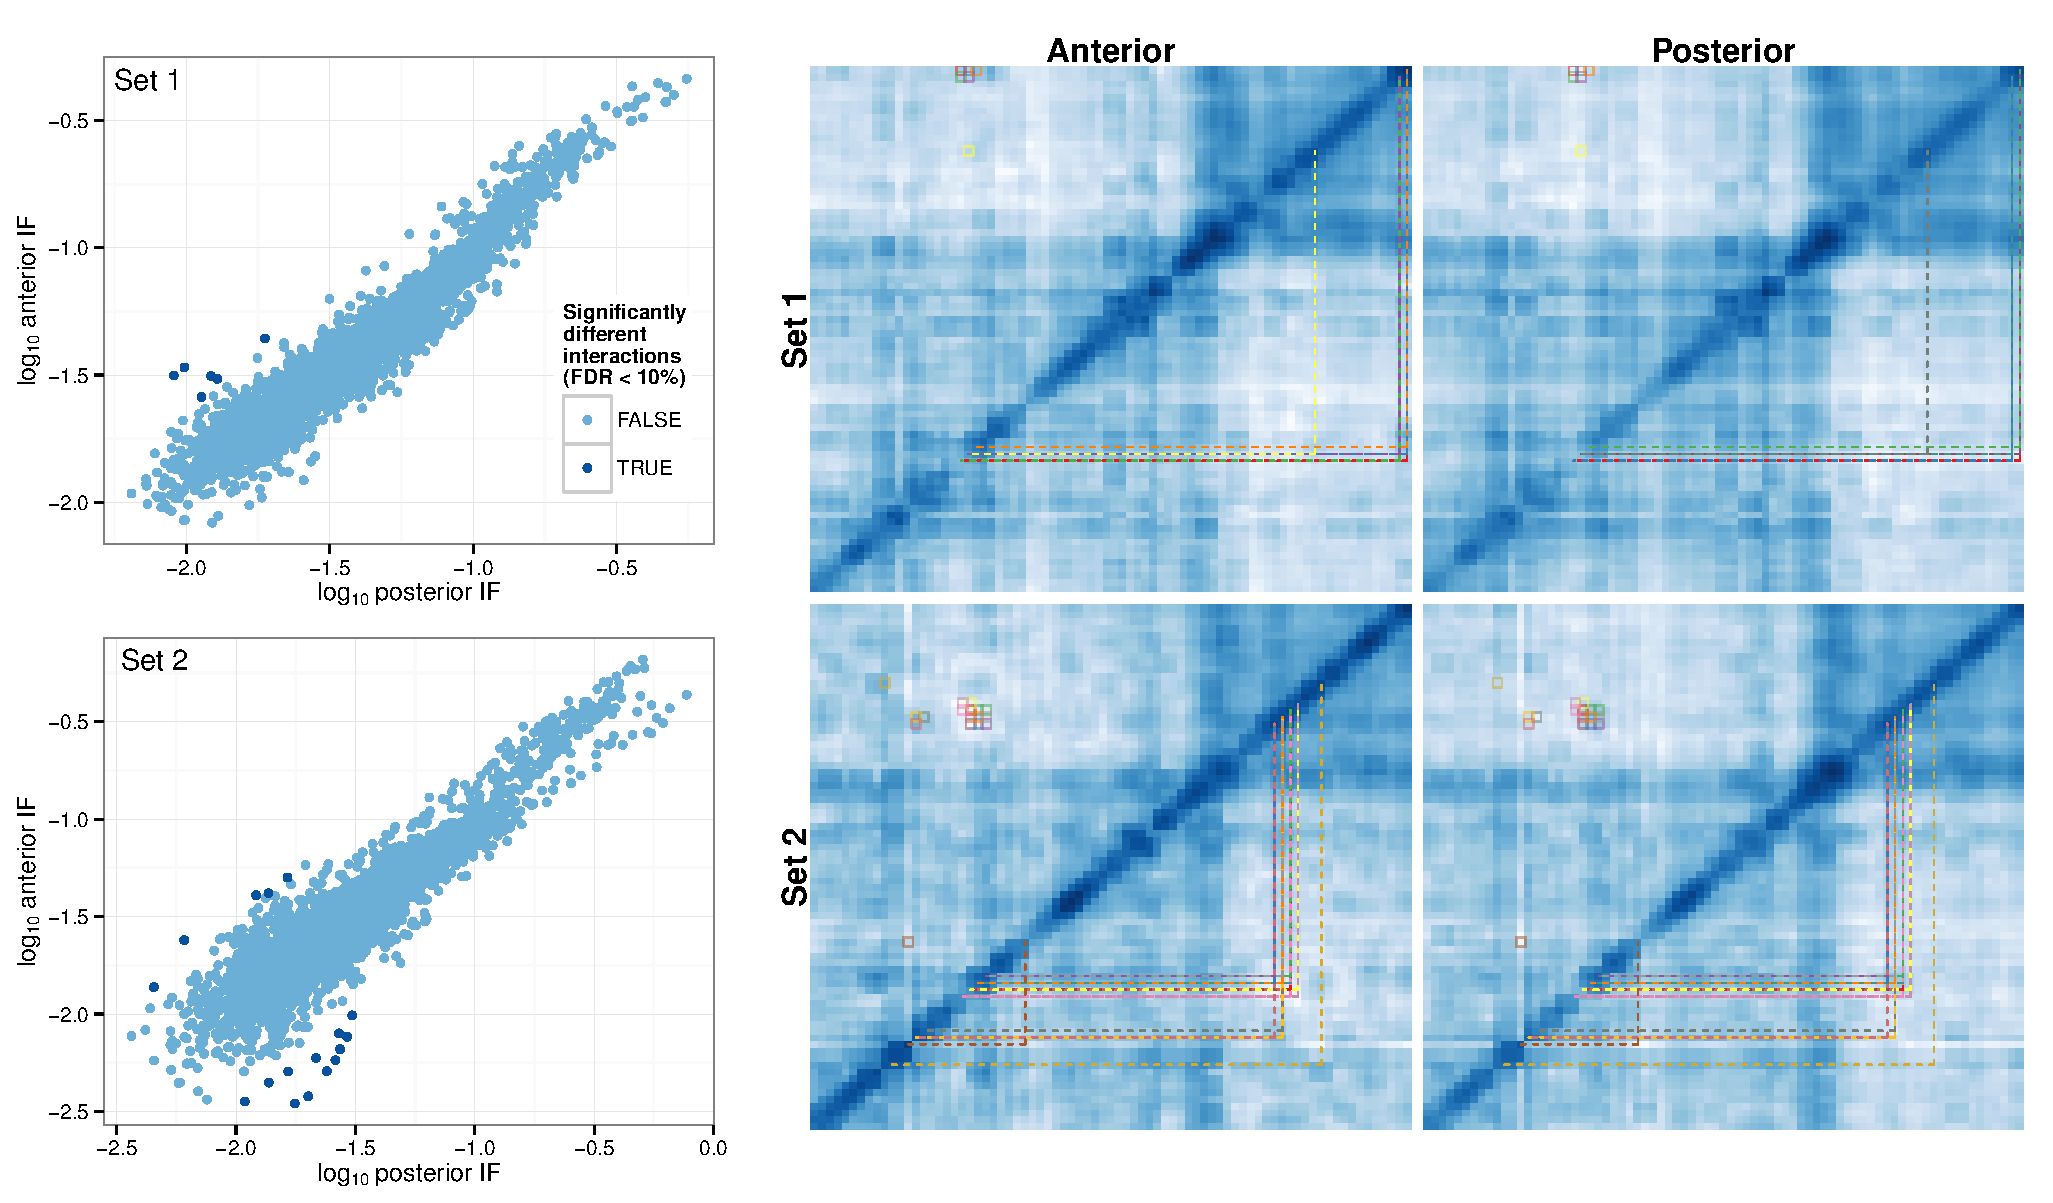
\includegraphics[width=\textwidth]{figs/5cdiff.pdf}
%\captionsetup{width=\textwidth} 
%\caption[Differential 5C contacts between 5C experiments over the HoxD locus in anterior and posterior limb bud cells.]{ {\bf Differential 5C contacts between 5C experiments over the HoxD locus in anterior and posterior limb bud cells. }
%Scatterplots compare anterior and posterior interaction frequencies ($IF$, \emph{left}) and significantly different contacts are highlighted in the 5C heatmaps with colour-matched lines and squares (\emph{right}). No differential contacts were found over both repeats (Sets 1 and 2).
%}\label{fig:5cdiff}
%\end{center} 
%\end{figure} 
%
%
%\subsection{5C / Hi-C comparison}
%
%% Precedent for comparing 5C and Hi-C : Phillips-Cremins2013
%
%\begin{figure}
%\begin{center} 
%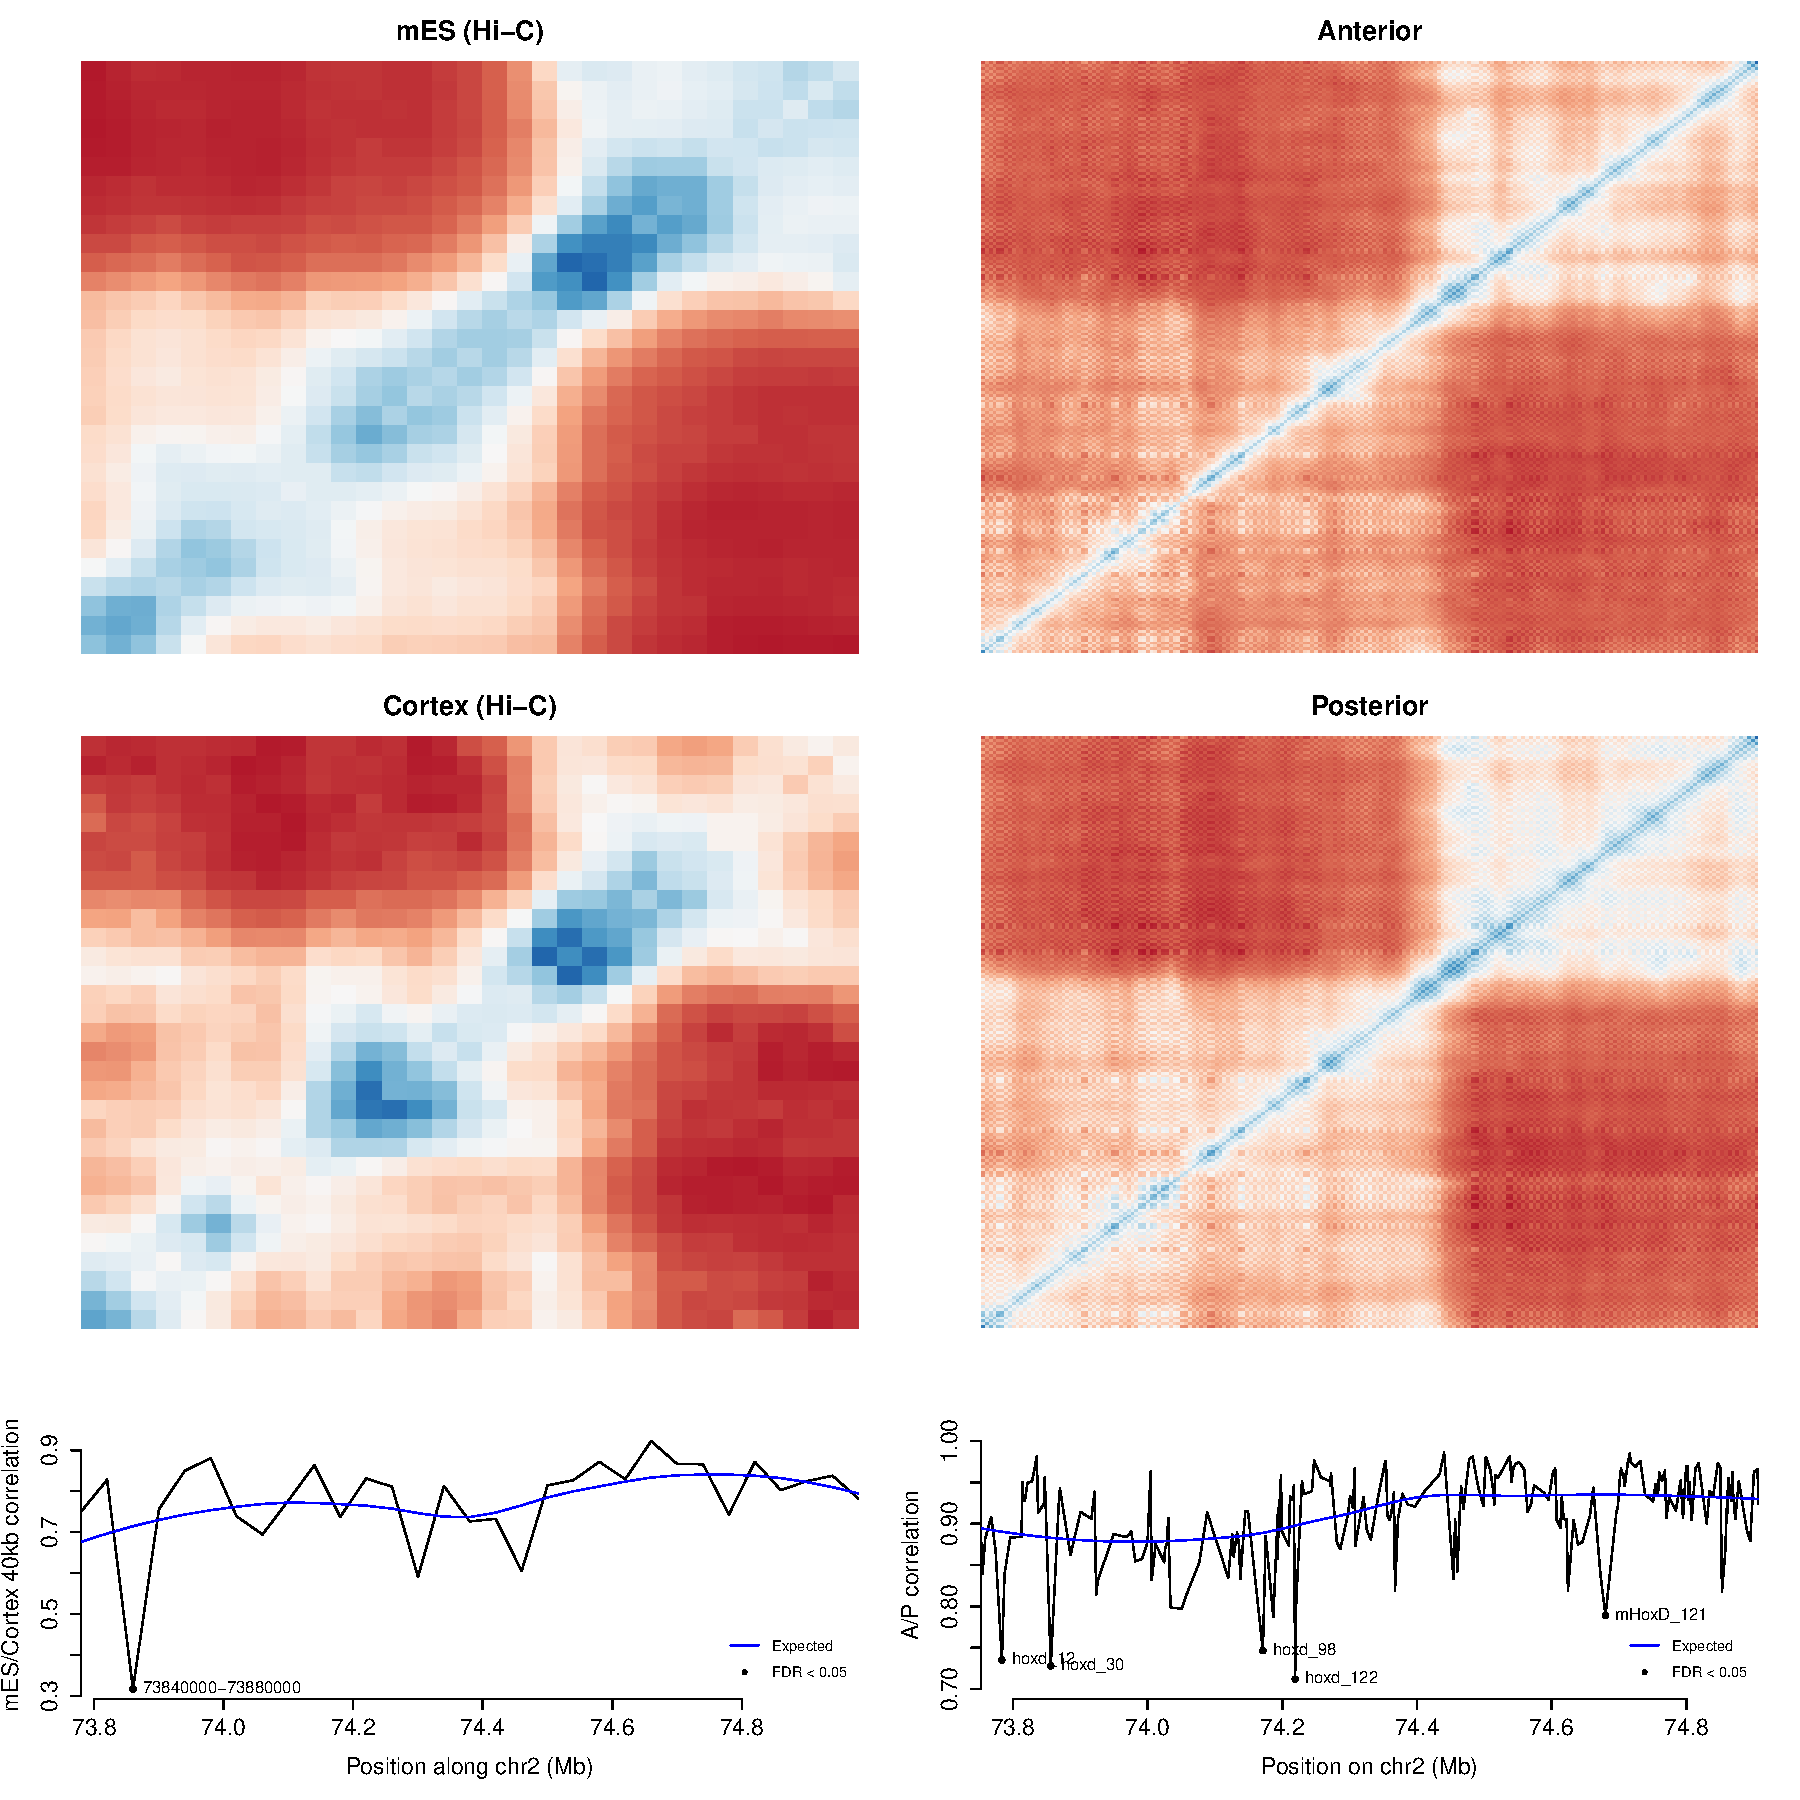
\includegraphics[width=\textwidth]{figs/5chic.pdf}
%\captionsetup{width=\textwidth} 
%\caption[Comparison of 5C and Hi-C over the HoxD region in different cell types.]{ {\bf Comparison of 5C and Hi-C over the HoxD region in different cell types. }
%Previously-published Hi-C data\cite{Dixon2012} for two cell types is shown alongside novel 5C data in limb bud lines. Chances in the total contacts for a row or column are shown (\emph{lower}) with a fitted loess model. Significance outliers are labelled.
%}\label{fig:5cdiff}
%\end{center} 
%\end{figure} 


\ifstandalone
\begin{small}
\bibliography{/Users/benmoore/Documents/library,/Users/benmoore/Documents/customrefs}
\end{small}
\fi

\end{document}
